\section{Normes $\L^p$}
\ref{normes_lp_et_inegalites}

\begin{marginfigure}
    \centering
    \begin{tikzpicture}[scale=2]
    \def\eps{0.3}
    \draw[thick, ->] (-1-\eps,0) -- (1+\eps,0); % node[below] {$x$};
    \draw[thick, ->] (0,-1-\eps) -- (0,1+\eps); % node[right] {$y$};
    \draw[thick, myblue] (0,0) circle (1);
    \draw[thick, myred] (-1,-1) rectangle (1,1);
    \draw[thick, mygreen, rotate=45] (-{sqrt(2)/2},-{sqrt(2)/2}) rectangle ({sqrt(2)/2},{sqrt(2)/2});

    \node[mygreen] at (45:{sqrt(2)/2}) {\contour{white}{$p=1$}};
    \node[myblue] at (45:1) {\contour{white}{$p=2$}};
    \node[myred] at (45:{sqrt(2)}) {\contour{white}{$p=\infty$}};

    \node[above] at (0,1+\eps) {$\big(\module{x}^p + \module{y}^p\big)^{1/p} = 1$};
    
    \node[below right] at (1,0) {$1$};
    \node[below left] at (-1,0) {$-1$};
    \node[below right] at (0,-1) {$-1$};
    \node[above left] at (0,1) {$1$};
\end{tikzpicture}
    \caption{Exemples (des frontières) de boules unités de $\R^2$}
\end{marginfigure}
\begin{defi}
Soient $p \in \N$ et $I$ une intervalle de $\R$. La fonction $f$ est de classe $\L^p$ sur $I$ si $f^p$ est intégrable sur $I$. On note alors
\[
\norm{f}_{\L^p} = \left(\int_I \module{f}^p\right)^{1/p}.
\]
On note $\L^p(I)$ l'ensemble des fonctions de classes $\L^p$ sur $I$.
\end{defi}

\begin{remarque}
Dans la suite de ce thème, on ne considère que des fonctions continues sur $I$. La positivité de l'intégrale assure alors que, si $\norm{f}_{\L^p} = 0$, alors $f$ est identiquement nulle sur $I$.
\end{remarque}

%-----------
\subsection{Limite $p \to +\infty$}

\begin{theo}
Soit $f$ une fonction continue sur le segment $\interff{a}{b}$. Alors,
\[
\lim_{p\to+\infty} \norm{f}_{\L^p} = \norm{f}_\infty.
\]
\end{theo}
Voir l'index des notations \ref{indexnotations} pour la définition de la norme $\norm{\,\cdot\,}_\infty$.
% \todoinline{Ajouter $\norm{\cdot}_\infty$ à un index des notations.}

% \begin{exercice}
    % \marginnote[0cm]{Source : \cite{acamanes} \href{https://acamanes.github.io/psi/psi_doc/exos_e01.pdf}{(Exercice 9. TD I)}}
    % Soit $f$ une fonction supposée continue et positive sur $\interff{a}{b}$. Étudier la suite de terme général 
    % $$u_n \defeq \left( \frac{1}{b-a} \int_{a}^{b} f(x)^n \d x \right)^{1/n}.$$
 % \end{exercice}


\begin{exercice}
Soit $f$ une fonction continue sur le segment $\interff{a}{b}$.
\begin{questions}
\item Montrer qu'il existe un réel $c_p$ tel que $\norm{f}_{\L^p} \leqslant c_p \norm{f}_\infty$.

\item Soit $\varepsilon > 0$. Montrer qu'il existe un segment $\interff{c}{d} \subset \interff{a}{b}$ tel que
\[
\forall x \in \interff{c}{d},\quad f(x) \geqslant \norm{f}_{\L^\infty} - \varepsilon.
\]

\item En déduire qu'il existe un réel $d_p$ tel que
\[
d_p \big(\norm{f}_\infty - \varepsilon\big) \leqslant \norm{f}_{\L^p}.
\]

\item Conclure.
\end{questions}
\end{exercice}

\begin{marginfigure}[-5cm]
    \centering
    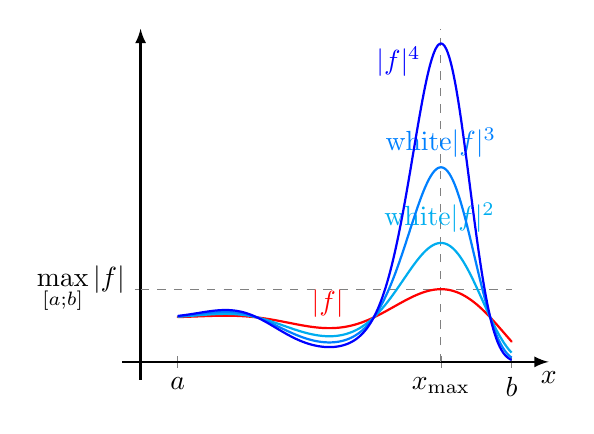
\begin{tikzpicture}
    \begin{axis}[
        width=7cm,
        xmin=-0.05, xmax=1.1,
        ymin=-0.4, ymax=7.5,
        axis lines=middle,
        axis line style=thick,
        axis line style={-latex},
        legend cell align={left}, 
        legend style={
            draw=none,
            fill=none,
            font=\footnotesize,
            legend image code/.code={\node[anchor=west] {#1};}
        },
        xtick={0.1, 0.8093645484949833, 1},
        xticklabels={$a$, $x_\mathrm{max}$, $b$},
        ytick={0, 1.6363476181939256},
        yticklabels={$0$, $\max\limits_{[a;b]} |f|$},
        xlabel=$x$,
        every axis x label/.style={at={(current axis.right of origin)},anchor=north},
    ];

    \draw[gray, dashed] (0,1.6363476181939256) -- (1,1.6363476181939256);
    \draw[gray, dashed] (0.8093645484949833,0) -- (0.8093645484949833,7.5);
    % Plot for n=1
    \addplot[domain=0.1:1, samples=200, color=red, smooth, thick, line join=round,line cap=round] {abs(x^2 * sin(10*deg(x))+1)} node[pos=0.2, above] {$|f|$};
    % \addlegendentry{\textcolor{blue!20!cyan}{$n = 1$}}

    % Plot for n=2
    \addplot[domain=0.1:1, samples=200, color=blue!0!cyan, smooth, thick] {abs(x^2 * sin(10*deg(x))+1)^2} node[pos=0.537, above] {\contour{white}{$|f|^2$}};
    % \addlegendentry{\textcolor{blue!40!cyan}{$n = 2$}}

    % Plot for n=3
    \addplot[domain=0.1:1, samples=200, color=blue!50!cyan, smooth, thick] {abs(x^2 * sin(10*deg(x))+1)^3} node[pos=0.533, above] {\contour{white}{$|f|^3$}};
    % \addlegendentry{\textcolor{blue!60!cyan}{$n = 3$}}

    % Plot for n=4
    \addplot[domain=0.1:1, samples=200, color=blue!100!cyan, smooth, thick] {abs(x^2 * sin(10*deg(x))+1)^4} node[pos=0.5, left] {$|f|^4$};
    % \addlegendentry{\textcolor{blue!80!cyan}{$n = 5$}}
    \end{axis}
\end{tikzpicture}

    \caption{$\fonctionligne[f]{x}{x^2\sin(10x)+1}$}
\end{marginfigure}

\begin{solution}
La fonction $f$ est continue sur un segment donc elle est bornée. Ainsi, $\norm{f}_\infty$ est bien définie.

\begin{reponses}
\item Comme, pour tout $t \in \interff{a}{b}$, $\module{f(t)} \leqslant \norm{f}_\infty$, la croissance de l'intégrale assure que
\[
\int_a^b \module{f(t)}^p \d t \leqslant \int_a^b \big(\norm{f}_\infty\big)^p \d t.
\]
On obtient ainsi la majoration demandée, avec $c_p = (b - a)^{1/p}$.

\item Comme $f$ est continue, elle atteint ses bornes sur $\interff{a}{b}$ et il existe un réel $x_0$ tel que $f(x_0) = \norm{f}_\infty$.

Toujours comme $f$ est continue, il existe un réel $\eta$ tel que pour tout $x \in \interff{a}{b}$,
\[
\module{x - x_0} \leqslant \eta \implies \module{f(x) - f(x_0)} \leqslant \varepsilon.
\]
En particulier, pour $x \in \interff{x_0-\eta}{x_0+\eta} \cap \interff{a}{b}$,
\[
f(x) \geqslant f(x_0) - \varepsilon = \norm{f}_\infty - \varepsilon.
\]
On note $\interff{c}{d} = \interff{x_0-\eta}{x_0+\eta} \cap \interff{a}{b}$.

\item En utilisant la croissance de l'intégrale, on obtient ainsi
\[
(d - c)^{1/p} \big(\norm{f}_\infty - \varepsilon\big) \leqslant \norm{f}_{\L^p}.
\]

\item D'après les questions précédentes, pour tout $p \in \N$ et pour tout $\varepsilon > 0$,
\[
(d - c)^{1/p} \big(\norm{f}_\infty - \varepsilon\big) \leqslant \norm{f}_{\L^p} \leqslant (b - a)^{1/p} \norm{f}_\infty.
\]

Comme cette propriété est vraie pour tout $\varepsilon > 0$, alors

\[
(d - c)^{1/p} \norm{f}_\infty \leqslant \norm{f}_{\L^p} \leqslant (b - a)^{1/p} \norm{f}_\infty.
\]

Enfin, comme $\lim\limits_{p\to+\infty} (d - c)^{1/p} = \lim\limits_{p\to+\infty} (b - a)^{1/p} = 1$, le \theoremeutilise{théorème d'encadrement}{theo:encadrement} permet de conclure.

% \item \textbf{Minoration:} soit $\varepsilon > 0$, soit $x_0$ tel que $f(x_0) = M$. Comme $f$ est continue en $x_0$, il existe $[c, d] \subset [a, b]$ tel que $x_0 \in [c, d]$ et pour tout $x \in [c, d]$, $f(x) \geqslant M - \varepsilon$ \emph{(un dessin permet de bien comprendre la stratégie)}.\\
        % On peut ensuite montrer que $u_n \geqslant \left(\frac{d-c}{b-a} \right)^{1/n}(M-\varepsilon) \xrightarrow[n \to + \infty]{} M-\varepsilon$.
        % \item Finalement, $u_n \displaystyle \longrightarrow M = \max_{[ a, b ]} f = \Ninf{f}$.
    % \end{itemize}
\end{reponses}
\end{solution}

\subsection{Limite $p \to 0$}

\begin{theo}
Soit $f \in \Cont\big(\mathopen{}\interff{0}{1},\Rpe\big)$. Alors,
\[
\lim_{p\to0} \norm{f}_{\L^p} = \exp\mathopen{}\left\{\int_0^1 \ln\mathopen{}\module{f(x)} \d x\right\}.
\]
\end{theo}

%---------------

\begin{exercice}%
Soit $f \in \Cont\big(\mathopen{}\interff{0}{1},\Re)$. On suppose que $f$ est à valeurs positives et on pose $I(y) = \int_0^1 f(x)^y \d x$.
\begin{questions}
\item Soit $g$ une fonction définie sur un voisinage de $0$ à valeurs dans $\Rpe$, dérivable en $0$, vérifiant $g(0) = 1$. Déterminer $\lim\limits_{y\to0} g(y)^{1/y}$.

\item Montrer que $I$ est une fonction dérivable sur $\Rp$.

\item En déduire que
\[
\lim_{y\to0} \mathopen{}\left(\int_0^1 f(x)^y \d x\right)^{1/y} = \exp\mathopen{}\left\{\int_0^1 \ln\mathopen{}\big(f(x)\big) \d x\right\}.
\]
\end{questions}
\end{exercice}

\begin{solution}
\begin{reponses}
\item Comme $g$ est dérivable, d'après le théorème de \nom{Taylor}--\nom{Young}\marginnote[-7pt]{\etoile{Théorème de \nom{Taylor}--\nom{Young}\index[theoremesutilises]{\nom{Taylor}--\nom{Young}}}}, $g(y) = 1 + y g'(0)~+~\petito(y)$. Ainsi,
\begin{align*}
g(y)^{1/y} &= \exp\mathopen{}\left\{\frac{1}{y} \ln(g(0) + y g'(0) + \petito(y))\right\}
= \exp\mathopen{}\left\{g'(0) + \petito(1)\right\}
\to \e^{g'(0)}.
\end{align*}

\item En posant $\fonctionligne[F]{(x, y)}{f(x)^y}$, alors
\[
\module{\frac{\partial F}{\partial y}(x, y)} = \module{\ln\mathopen{}\big(f(x)\big) f(x)^y}.
\]

La fonction $\ln \circ\, f$ est continue sur le segment $\interff{0}{1}$ donc elle est bornée par une constante $M$. Ainsi,
\begin{align*}
\module{F(x, y)} &\leqslant \e^{a M},\\
\module{\frac{\partial F}{\partial y}(x, y)} &\leqslant M \e^{a M}.
\end{align*}

D'après le \theoremeutilise{théorème de dérivation sous le signe intégral}{theo:derivationsoussigneintegrale}, la fonction $I$ est dérivable sur $\interfo{0}{1}$ et
\begin{align*}
I'(y) &= \int_0^1 \ln\mathopen{}\big(f(x)\big) f(x)^y \d x \\
I'(0) &= \int_0^1 \ln\mathopen{}\big(f(x)\big) \d x
\end{align*}

\item Finalement,
\[
\lim_{y\to0} \mathopen{}\left(\int_0^1 f(x)^y \d x\right)^{1/y} = \exp\mathopen{}\left\{\int_0^1 \ln\mathopen{}\big(f(x)\big) \d x\right\}.
\]
\end{reponses}
\end{solution}

\url{https://math.stackexchange.com/questions/2351581/convergence-question-about-lp-norm-when-p-tends-to-zero}


%-----------
\subsection{Cas $p \geqslant 1$}

Lorsque l'exposant $p$ satisfait $0 < p < 1$, on constate que l'inégalité triangulaire ne peut pas être satisfaite par $\norm{\,\cdot\,}_{\L^p}$, ce qui justifie, pour bénéficier d’une structure naturelle d’espace vectoriel, de se restreindre à supposer $1 < p < +\infty$.

\begin{theo}[Inégalité de \nom{Minkowski}]
Soit $p \geqslant 1$. Si $f$ et $g$ sont deux fonctions appartenant à $\L^p(I)$, alors
\[
\norm{f + g}_{\L^p} \leqslant \norm{f}_{\L^p} + \norm{g}_{\L^p}.
\]
Ainsi, $\L^p(I)$ est un espace vectoriel et $\norm{\,\cdot\,}_{\L^p}$ est une norme.
\end{theo}

\begin{remarque}
Les cas $p = 1$ et $p = +\infty$ sont aisément vérifiables. On se limite par la suite au cas $1 < p < +\infty$.
\end{remarque}

Cette inégalité repose sur le théorème suivant :
\begin{theo}[Inégalité de \nom{Hölder}]
Soient $1 < p,\, q < +\infty$, $q$ tels que $\frac{1}{p} + \frac{1}{q} = 1$ et $f,\, g$ deux fonctions à valeurs strictement positives. Si $f$ appartient à $\L^p(I)$ et $g \in \L^q(I)$, alors $f g$ appartient à $\L^1(I)$ et
\[
\int_I f g \leqslant \norm{f}_{\L^p} \norm{g}_{\L^q}.
\]
\end{theo}

\begin{remarque}
Lorsque $p = 2$, alors $q = 2$ et on retrouve l'\theoremeutilise{inégalité de \nom{Cauchy}--\nom{Schwarz}}{theo:inegalitecs}.
\end{remarque}

\begin{exercice}
Les cas où $\norm{f}_{\L^p} = 0$ ou $\norm{g}_{\L^q} = 0$ sont triviaux. On se limite donc au cas où ces quantités sont non nulles et on pose
\[
F = \frac{f}{\norm{f}_{\L^p}}
\quad \text{et} \quad
G = \frac{g}{\norm{g}_{\L^q}}.
\]
Soit $x \in I$.
\begin{questions}
\item Montrer qu'il existe deux réels $s$ et $t$ tels que $F(x) = \e^{t/p}$ et $G(x) = \e^{s/q}$.

\item Montrer que $\e^{\frac{s}{p} + \frac{t}{q}} \leqslant \frac{1}{p} \e^s + \frac{1}{q} \e^t$.

\item En déduire l'inégalité de \nom{Hölder}.
\end{questions}
\end{exercice}

\begin{solution}
\begin{reponses}
\item Pour tout $x$ réel, $F(x)$ et $G(x)$ sont deux réels strictement positifs, on pose $t~=~p \ln\mathopen{}\big(F(x)\big)$ et $s = q \ln\mathopen{}\big(G(x)\big)$.

\item Rappelons que $\frac{1}{p} + \frac{1}{q} = 1$. Pour tous $s$ et $t$ réels, comme la fonction exponentielle est convexe, d'après l'\theoremeutilise{inégalité de \nom{Jensen}}{theo:inegalitejensen},
\[
\e^{\frac{s}{p} + \frac{t}{q}} \leqslant \frac{1}{p} \e^s + \frac{1}{q} \e^t.
\]

\item Alors,
\begin{align*}
F(x) G(x) &\leqslant \frac{1}{p} F(x)^p + \frac{1}{q} G(x)^q
\end{align*}
Comme $F^p$ et $G^q$ sont intégrables, alors $F G$ est intégrable et
\[
\int_I F G \leqslant \frac{1}{p} + \frac{1}{q} = 1.
\]
La linéarité de l'intégrale permet alors de conclure.
\end{reponses}
\end{solution}

\begin{exercice}
Soit $f$ et $g$ deux fonctions de classe $\L^p$ sur $I$.
\begin{questions}
\item Montrer que $\module{f + g}^p \leqslant 2^p \module{f}^p + 2^p \module{g}^p$.

\item En déduire que $(f + g) \in \L^p(I)$.

\item En décomposant $(f + g)^p = f (f + g)^{p-1} + g (f + g)^{p-1}$, en déduire l'inégalité de \nom{Minkowski}.
\end{questions}
\end{exercice}

\begin{solution}
\begin{reponses}
\item Pour tout $x \in I$,
\begin{itemize}
\item soit $\module{f(x)} \leqslant \module{g(x)}$ et $\module{f(x) + g(x)}^p \leqslant 2^p \module{g(x)}^p$,
\item soit $\module{g(x)} \leqslant \module{f(x)}$ et $\module{f(x) + g(x)}^p \leqslant 2^p \module{f(x)}^p$.
\end{itemize}
Ainsi, dans tous les cas,
\[
\module{f + g}^p \leqslant 2^p \module{f}^p + 2^p \module{g}^p.
\]

\item D'après la question précédente et le \theoremeutilise{théorème de comparaison des intégrales}{theo:comparaison}, $f + g~\in~\L^p(I)$.

\item En utilisant la décomposition proposée, on remarque que
\begin{align*}
\big(\mathopen{}\module{f + g}^{p-1}\big)^q
&= \module{f + g}^{q(p-1)}
= \module{f + g}^p.
\end{align*}
Ainsi, $\module{f + g}^{p-1} \in \L^q(I)$.

En appliquant deux fois l'inégalité de \nom{Hölder},
\begin{align*}
\norm{f + g}_{\L^p}^p
&= \norm{|f| \cdot |f + g|^{p-1}}_{\L^1}
+ \norm{|g| \cdot |f + g|^{p-1}}_{\L^1}\\
&\leqslant \norm{f}_{\L^p}^p \norm{f + g}_{\L^p}^{p/q}
+ \norm{g}_{\L^p}^p \norm{f + g}_{\L^p}^{p/q}\\
&\leqslant \norm{f + g}_{\L^p}^{p/q} \big(\norm{f}_{\L^p} + \norm{f}_{\L^q}\big).
\end{align*}

On conclut en simplifiant par $\norm{f + g}_{\L^p}^{p/q}$.
\end{reponses}
\end{solution}

% \todoinline{Pointer vers
% Exercice 2 de \url{https://www.imo.universite-paris-saclay.fr/~joel.merker/Enseignement/Integration/l-p-espaces.pdf}}
% \begin{exercice}
    % On considère les espaces $\L^p(\R^d)$ pour  $0 < p < +\infty$. Montrer que si l'on a 
    % \[
    % \norm{f + g}_{\L^p} \leqslant  \norm{f}_{\L^p} + \norm{g}_{\L^p}
    % \]
    % pour toutes fonctions $f, g \in \L^p(\R^d )$, alors nécessairement $p \geqslant 1$.
% \end{exercice}

%-----------
\subsection{Inclusions entre les $\L^p$}

\begin{theo}
Si $I$ est un intervalle borné, on note $|I|$ sa longueur. Pour tout $p < q$, $\L^q(I) \subset \L^p(I)$ et $\|f\|_p \leqslant \module{I}^{\frac{1}{p} - \frac{1}{q}} \norm{f}_{\L^q}$.
    % Si $\Omega$ est de mesure $\module{\Omega}$ finie, alors pour $p<q$, $\L^q(\Omega) \subset \L^p(\Omega)$ et pour tout $f \in \L^q(\Omega)$, $\norm{f}_{\L^p} \leqslant \module{\Omega}^{\frac{1}{p} - \frac{1}{q}} \norm{f}_{\L^q}$.
\end{theo}

\begin{demo}
Comme $I$ est borné, alors la fonction constante égale à $1$ appartient à tous les espaces $\L^q$. Ainsi, d'après l'inégalité de \nom{Hölder},
\begin{align*}
\norm{f}_{\L^p}^p
&\leqslant \left(\int_I \module{f}^q\right)^{p/q} \left(\int_I 1\right)^{1-p/q}
\leqslant \norm{f}_{\L^q}^p \cdot \module{I}^{1-p/q}.
\end{align*}
\end{demo}

\begin{remarque}
En utilisant des intégrales de \nom{Riemann}, on montre que ces inclusions sont fausses dès que $I$ n'est pas borné. \\
En effet, choisissons $p$ et $q$ tels que $p > q$ et considérons $\alpha > 0$ avec la fonction $f(x) = \frac{1}{1+\module{x}^\alpha}$ pour $x \in \R$. Si on choisit $1/p < \alpha < 1/q$, alors $f \in \L^p(\R)$ mais $f \not\in \L^q(\R)$, donc $\L^p(\R) \not\subset \L^q(\R)$. \\
Considérons maintenant la fonction $g(x) = \frac{1}{\module{x}^\alpha (1+x^2)}$ pour $x \in \R$. Si on choisit encore $\alpha$ tel que $1/p <  \alpha < 1/q$, alors $g \in \L^q(\R)$ mais $g \not\in \L^p(\R)$, donc $\L^q(\R) \not\subset \L^p(\R)$.\\
Des résultats plus précis concernant les inclusions entre espaces $\L^p$ peuvent être trouvés dans~\cite{rudin2009}.
\end{remarque}